\subsubsection{Compito C1: Registrazione e inserimento dati accademici}
Il compito C1 prevedeva il completamento della procedura di registrazione alla piattaforma, comprensiva dell'inserimento delle credenziali di accesso e dei dati accademici (Università, Dipartimento e Corso di studi). L'obiettivo di questo compito era valutare l'usabilità del form di registrazione, verificando l'effettiva riduzione degli errori sistematici riscontrati nella versione originale attraverso l'introduzione di un form multi-step guidato (wizard) nella versione riprogettata.

\paragraph{Analisi delle prestazioni generali}
Come si evince dalla Tabella~\ref{tab:6-c1-1}, il tasso di completamento (Success Rate) si è attestato al 100\% per entrambe le versioni del sistema. I dati rilevano un abbattimento dell'80,00\% nella media degli errori e una contrazione della mediana dei click (-15,79\%) a favore della versione riprogettata. Di contro, si osserva un incremento del 14,29\% nella mediana del tempo di esecuzione per la versione B.

\begin{table}[H]
	\centering
	\small
	\renewcommand{\arraystretch}{1.2}
	\caption{Metriche prestazionali globali aggregate per il compito C1.}
	\label{tab:6-c1-1}
	\begin{tabular}{|l|c|c|c|}
		\hline
		\rowcolor{gray!30}
		\textbf{Metrica} & \textbf{Versione originale (A)} & \textbf{Versione post-riprogettazione (B)} & \textbf{Variazione} \\ \hline
		Success Rate     & 100,00\%                        & 100,00\%                                   & 0,00\%              \\ \hline
		Media Errori     & 1,00                            & 0,20                                       & -80,00\%            \\ \hline
		Mediana Tempo    & 1:10.00                         & 1:20.00                                    & 14,29\%             \\ \hline
		Mediana Click    & 19                              & 16                                         & -15,79\%            \\ \hline
		Media Difficoltà & 1,33                            & 1,20                                       & -10,00\%            \\ \hline
	\end{tabular}
\end{table}

La significativa riduzione del numero medio di errori e di click complessivi trova giustificazione nella riorganizzazione strutturale dell'interfaccia di input. L'introduzione della validazione contestuale e di indicatori chiari di avanzamento ha permesso di prevenire gli errori di inserimento tipici della versione originale. L'aumento del tempo mediano di completamento nella versione riprogettata è direttamente riconducibile alla nuova struttura a step e all'inserimento di una schermata di riepilogo finale. Tale scelta progettuale privilegia deliberatamente l'accuratezza dei dati inseriti rispetto alla rapidità di esecuzione, aumentando le probabilità di esiti positivi durante la compilazione del form e limitando la necessità di correzioni successive.

\paragraph{Analisi qualitativa: commenti e osservazioni degli utenti}

I dati quantitativi trovano un forte riscontro qualitativo nelle annotazioni degli sperimentatori e nei commenti espliciti rilasciati dagli utenti durante il test (\textit{thinking aloud}).

Per la versione originale (A), sono emerse diverse criticità ricorrenti:

\begin{itemize}
	\item \textbf{Coerenza linguistica}: molti utenti hanno lamentato la presenza della lingua inglese nel form di registrazione. Questo ha generato confusione sul significato di alcuni pulsanti. Tale problematica rappresenta una netta violazione del principio di coerenza linguistica con il resto della piattaforma in italiano.

	\item \textbf{Effetto ``Flash'' e distrazione}: diversi partecipanti hanno segnalato un forte fastidio causato da un ``effetto flash'' (la schermata diventava completamente bianca per qualche milli-secondo) durante la compilazione. Questo bug visivo si è rivelato un grave elemento di distrazione: in più occasioni ha indotto l'utente a dimenticare di selezionare campi obbligatori (come il corso di studio). La situazione è stata aggravata dalla totale assenza di messaggi di errore chiari e tempestivi al momento del salvataggio.

	\item \textbf{Mancanza di visibilità dello stato}: è emersa un'esplicita frustrazione legata all'impossibilità di visualizzare in chiaro la password digitata. Questa criticità giustifica pienamente l'implementazione del pattern \textit{Password Strength Meter} (con l'apposito \textit{toggle} per la visibilità) introdotto nella versione B.

	\item \textbf{Navigazione iniziale}: il flusso per raggiungere il form di registrazione dalla homepage è stato giudicato a tratti poco intuitivo, con alcuni utenti che si aspettavano opzioni esplicite come ``non ho un account'' direttamente nella schermata di login.
\end{itemize}

Passando alla versione post-riprogettazione (B), le considerazioni generali sono mutate radicalmente in positivo, confermando il successo delle scelte di design adottate:

\begin{itemize}
	\item \textbf{Apprezzamento per il Riepilogo}: la novità più elogiata in assoluto è stata l'introduzione dello step finale, rinominato in ``Riepilogo'' (invece del generico ``Fatto''). Molti utenti hanno esplicitamente apprezzato questa schermata. L'apprezzamento deriva dal fatto che ha restituito loro il controllo sui dati accademici prima della conferma finale.

	\item \textbf{Linearità del flusso}: l'approccio strutturato in step progressivi ha reso il compito percepito come ``più lineare''.

	\item \textbf{Innalzamento delle aspettative}: l'impatto dei miglioramenti è perfettamente sintetizzato dal commento di un utente (sottoposto all'ordine B-A) che, dopo aver completato il compito sulla nuova interfaccia, ha ammesso: ``Se avessi visto questo prima, sarei stato più cattivo con la versione A''. Ciò dimostra come il nuovo design abbia innalzato le aspettative di usabilità, rendendo evidenti e intollerabili i difetti della versione precedente.
\end{itemize}

\paragraph{Valutazione dell'effetto di apprendimento}
Analizzando i dati in base all'ordine di esecuzione, emergono variazioni significative nei tempi di completamento. Per il gruppo sottoposto all'ordine A-B, si osserva un tempo mediano maggiore nella versione originale, che si riduce notevolmente durante l'utilizzo della versione B. Nel gruppo associato all'ordine B-A, l'esperienza pregressa maturata sulla versione riprogettata ha abbattuto il tempo necessario per completare il medesimo compito sulla versione originale. Questo risultato evidenzia un trasferimento positivo della conoscenza delle operazioni richieste, che ha parzialmente compensato i limiti strutturali e la mancanza di feedback della variante originale.

\begin{figure}[H]
	\centering
	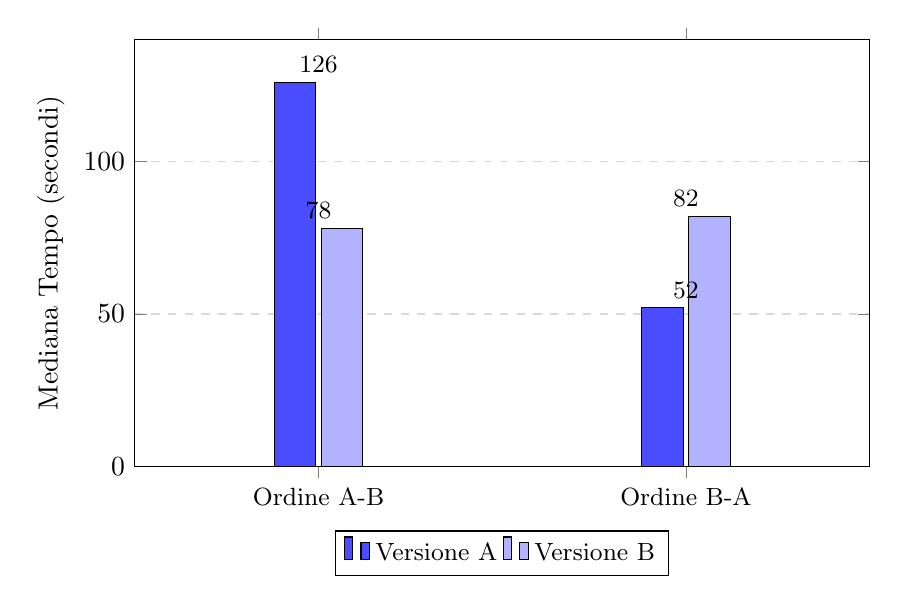
\begin{tikzpicture}
		\begin{axis}[
				ybar,
				bar width=15pt,
				width=0.9\textwidth,
				height=7cm,
				symbolic x coords={Ordine A-B, Ordine B-A},
				xtick=data,
				x tick label style={font=\small},
				ylabel={Mediana Tempo (secondi)},
				ymin=0, ymax=140,
				ymajorgrids=true,
				grid style={dashed, gray!30},
				enlarge x limits=0.5,
				legend style={at={(0.5,-0.15)}, anchor=north, legend columns=-1, font=\small},
				nodes near coords,
				every node near coord/.style={font=\small, color=black},
			]
			\addplot+[ybar, fill=blue!70, draw=black] coordinates {(Ordine A-B,126) (Ordine B-A,52)};
			\addplot+[ybar, fill=blue!30, draw=black] coordinates {(Ordine A-B,78) (Ordine B-A,82)};
			\legend{Versione A, Versione B}
		\end{axis}
	\end{tikzpicture}
	\caption{Confronto dei tempi mediani (in secondi) per il compito C1 in base all'ordine.}
	\label{fig:6-c1-1}
\end{figure}
